\documentclass[../../rapport.tex]{subfiles}

\begin{document}
  Cette section est un retour d'expérience sur l'utilisation de Lean en tant qu'outil de formalisation pour les
  mathématiques.

  Durant ce TER, j'ai donc utilisé Lean pour formaliser le théorème de Bowen, dont un preuve figure dans mon rapport de stage
  en annexe (preuve initialement dûe à R. Bowen).
  Ce théorème établit l'existence et l'unicité d'une certaine mesure de probabilité dite de Gibbs sur un espace métrique particulier,
  et donc ce théorème fait intervenir notamment de la topologie et de la théorie de la mesure.

  Pour formaliser ce théorème, j'ai donc eu recours à des outils extérieurs à Lean comme
  % \href{https://github.com/PatrickMassot/leanblueprint}{leanblueprint},
  leanblueprint (\textsc{Ajouter lien})
  qui permet à partir d'un texte mathématiques d'obtenir un graphe décrivant les liens entre les différents lemmes,
  théorèmes et définitions intermédiaires et d'en donner l'état d'avancement dans le code Lean associé.

  \begin{figure}[h]
    \centering
    \begin{subfigure}{.55\textwidth}
      \centering
      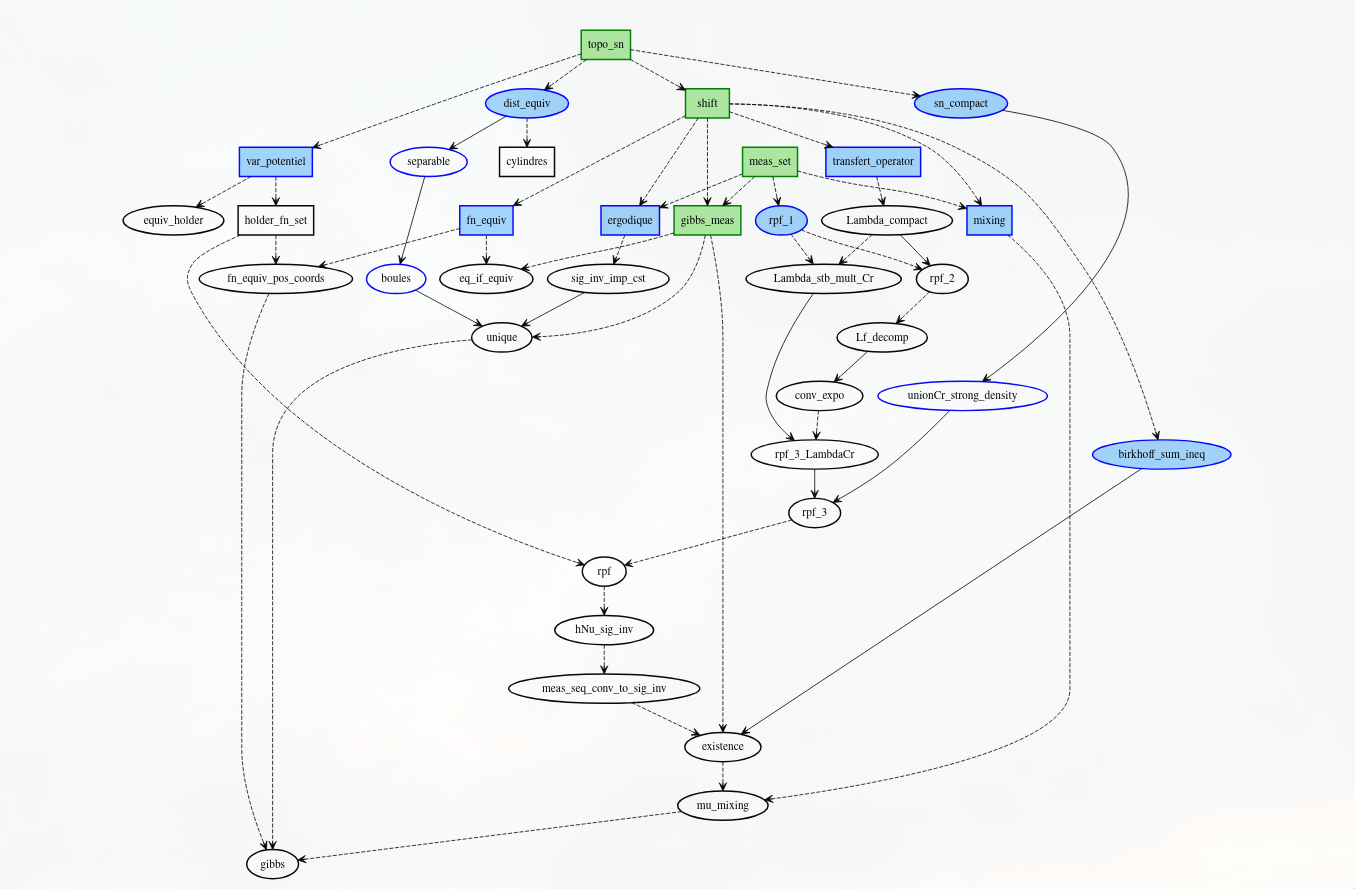
\includegraphics[width=.98\linewidth]{graph_1.png}
      \caption{État initial du graphe}
    \end{subfigure}
    \begin{subfigure}{.43\textwidth}
      \centering
      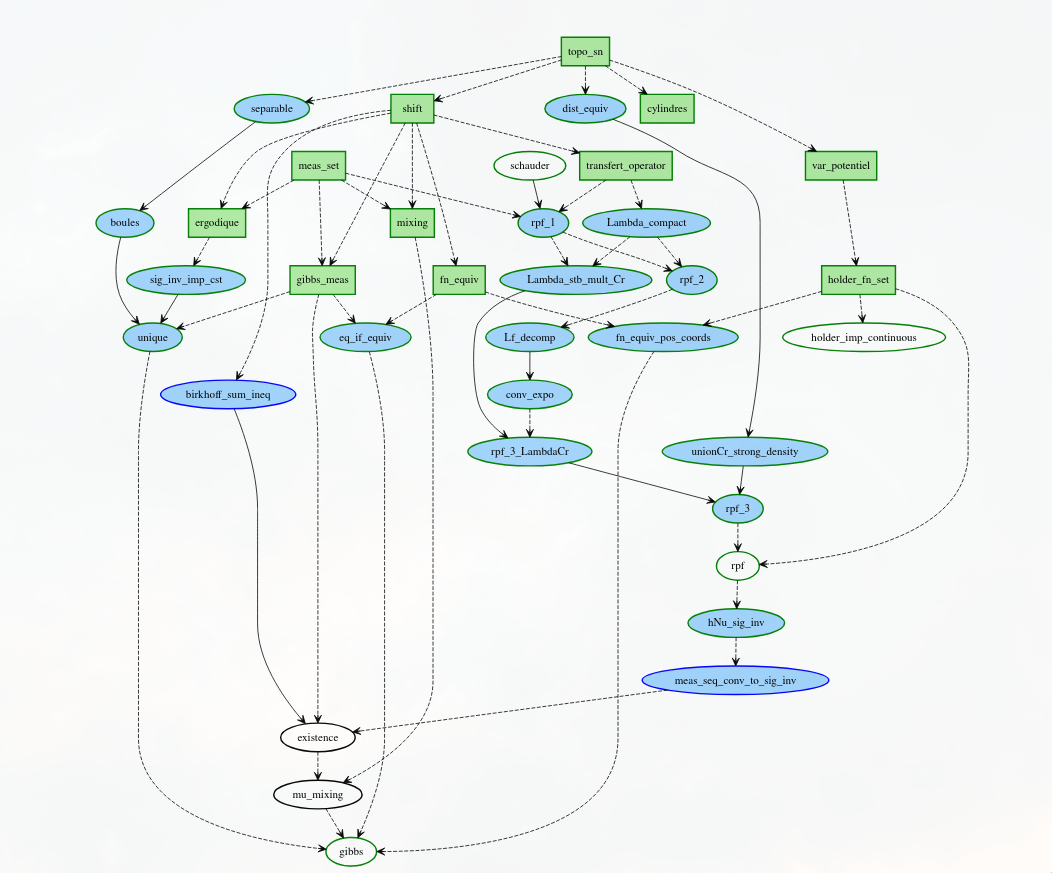
\includegraphics[width=.98\linewidth]{graph_8.png}
      \caption{État final du graphe}
    \end{subfigure}
  \end{figure}

  Les cases rectangulaires sont les définitions, les ellipses sont les lemmes, théorèmes, corollaires et propositions.
  Les couleurs en fond indiquent l'état d'avancement des preuves :
  le vert foncé pour pour les lemmes prouvés et dont les parents sont également prouvés,
  le vert clair pour les lemmes prouvés
  et le bleu pour les lemmes prêt à être prouvés (\textit{ie.} toutes les définitions nécessaires sont formalisés).
  Enfin les couleurs des bordures indiquent l'état d'avancement des énoncés des lemmes et des définitions :
  le vert pour les cases dont l'énoncé est formalisé
  et le bleu pour les cases dont l'énoncé n'est pas formalisé mairs prêt à l'être.

\end{document}
